\ifx\PREAMBLE\undefined
\documentclass{report}
\usepackage[format = hang, font = bf]{caption}
% The following is needed in order to make the code compatible
% with both latex/dvips and pdflatex. Added for using UML generated by MetaUML.
\ifx\pdftexversion\undefined
\usepackage[dvips]{graphicx}
\else
\usepackage[pdftex]{graphicx}
\DeclareGraphicsRule{*}{mps}{*}{}
\fi
\usepackage{array}
\usepackage{amsmath}
\usepackage{amsthm}
\usepackage{mathtools}
\usepackage{boxedminipage}
\usepackage{listings}
\usepackage{makecell}%diagonal line in table
\usepackage{float}%allowing forceful figure[H]
\usepackage{xcolor}
\usepackage{amsfonts}%allowing \mathbb{R}
\usepackage{amssymb}
\usepackage{alltt}
\usepackage{algorithmicx}
\usepackage[chapter]{algorithm} 
%chapter option ensures that algorithms are numbered within each chapter rather than in the whole article
\usepackage[noend]{algpseudocode} %If end if, end procdeure, etc is expected to appear, remove the noend option
\usepackage{xspace}
\usepackage{color}
\usepackage{url}
\def\UrlBreaks{\do\A\do\B\do\C\do\D\do\E\do\F\do\G\do\H\do\I\do\J\do\K\do\L\do\M\do\N\do\O\do\P\do\Q\do\R\do\S\do\T\do\U\do\V\do\W\do\X\do\Y\do\Z\do\[\do\\\do\]\do\^\do\_\do\`\do\a\do\b\do\c\do\d\do\e\do\f\do\g\do\h\do\i\do\j\do\k\do\l\do\m\do\n\do\o\do\p\do\q\do\r\do\s\do\t\do\u\do\v\do\w\do\x\do\y\do\z\do\0\do\1\do\2\do\3\do\4\do\5\do\6\do\7\do\8\do\9\do\.\do\@\do\\\do\/\do\!\do\_\do\|\do\;\do\>\do\]\do\)\do\,\do\?\do\'\do+\do\=\do\#\do\-}
\usepackage[breaklinks = true]{hyperref}
\lstset{
language = C++, 
showspaces = false,
breaklines = true, 
tabsize = 2, 
numbers = left, 
extendedchars = false, 
basicstyle = {\ttfamily \footnotesize}, 
keywordstyle=\color{blue!70}, 
commentstyle=\color{gray}, 
frame=shadowbox, 
rulesepcolor=\color{red!20!green!20!blue!20}, 
numberstyle={\color[RGB]{0,192,192}}, 
moredelim=[is][\underbar]{_}{_}
}
\mathchardef\myhyphen="2D
% switch-case environment definitions
\algblock{switch}{endswitch} 
\algblock{case}{endcase}
%\algrenewtext{endswitch}{\textbf{end switch}} %If end switch is expected to appear, uncomment this line.
\algtext*{endswitch} % Make end switch disappear
\algtext*{endcase}
\algnewcommand\algorithmicinput{\textbf{input:}}
\algnewcommand\Input{\item[\algorithmicinput]}
\algnewcommand\algorithmicoutput{\textbf{output:}}
\algnewcommand\Output{\item[\algorithmicoutput]}
\allowdisplaybreaks
\newtheorem{theorem}{Theorem}[chapter]
\newtheorem{corollary}[theorem]{Corollary}
\newtheorem{lemma}[theorem]{Lemma}
\newtheorem{definition}{Definition}[chapter]
\begin{document}
\fi
\chapter{NP Completeness}
Up to now we have been focusing on problems that can be solved in polynomial time. However, many important problems seem impossible to solve efficiently.  We will introduce NP-completeness to formalize the computational intractability of these problems, and introduce some algorithmic approaches to NP-complete problems. We will discuss only deterministic algorithms, but it does not affect the correctness of the conclusions drawn from our discussion: it is not likely that a problem requiring exponential time with deterministic algorithm can be solved by a randomized algorithm in polynomial time.
\section{NP Complete Problems}
\subsection{The Class P}
\begin{definition}
A problem is \textbf{polynomial-time solvable} if there is an algorithm that correctly solves it in $O(n^k)$ time for some constant $k$. $n$ is the length of the input.
\end{definition}
\begin{definition}
The class \textbf{P} is defined as the set of all polynomial-time solvable problems. 
\end{definition}
Every problem we've seen in the course is in the class P except for the cycle-free shortest path problem for graphs with negative cycles, as well as the knapsack problem. Knapsack problem is not polynomial-time solvable because its running time is $O(nW)$, while the input length is proportional to $\log W$. 
\subsection{Reductions and Completeness}
Computational intractability can be illustrated via relative difficulty, i.e. by showing that a problem is ``as hard as'' a lot of other problems. This requires the definition of reduction. 
\begin{definition}
Problem $\Pi_1$ \textbf{reduces} to problem $\Pi_2$ if given a polynomial time subroutine to solve $\Pi_2$, $\Pi_1$ can be solved in polynomial time based on it.
\end{definition}
Suppose $\Pi_1$ reduces to $\Pi_2$. If $\Pi_2\in P$, then $\Pi_1\in P$. The contrapositive is also correct: if $\Pi_1\notin P$, then $\Pi_2\notin P$, i.e. $\Pi_2$ is at least as hard as $\Pi_1$. 
\begin{definition}
Let C be a set of problems. A problem $\Pi$ is C-complete if 
\begin{enumerate}
\item $\Pi\in C$;
\item Every problem in C reduces to $\Pi$. 
\end{enumerate}
\end{definition}
A C-complete problem is the hardest problem in C.
\subsection{Traveling Salesman Problem}
\begin{description}
\Input{A completed undirected graph with non-negative edge costs.}
\Output{A minimum cost tour, i.e. a cycle that visits every vertex exactly once with minimum total cost.}
\end{description}
It has been conjectured for a long time that there exists no polynomial-time algorithm for the TSP problem. In order to demonstrate its computational intractability, we would like to show that it is C-complete for a really big set C. C cannot be the set of all problems. For instance, the Halting problem, i.e. given a program and an input for it, determine whether it will halt, has been proved to be unsolvable with any algorithm. TSP is obviously solvable in finite time via brute-force search. A less ambitious yet more promising idea is to try to prove that TSP is as hard as all brute-force solvable problems.
\subsection{The Class NP}
\begin{definition}
A problem is in the class NP\footnote{NP stands for ``nondeterministic polynomial'', instead of ``not polynomial''.} if
\begin{enumerate}
\item Solutions always have length polynomial in the input size;
\item Purported solutions can be verified in polynomial time. 
\end{enumerate} 
\end{definition}
As an example, looking for a TSP tour with total cost smaller than $T$ is an NP problem. The original TSP problem reduces to this problem via binary search over the threshold $T$. Also, constraint satisfaction problems, e.g. the 3SAT problem, are NP problems.  

The definition of NP ensures that each problem in NP can be solved by brute-force search in exponential time. The first condition implies that the number of candidate solutions is at most exponential in the input size. According to the second condition, each candidate can be verified in polynomial time, thus brute-force search takes at most exponential time. 

The two conditions in the definition of NP are quite weak, thus NP is a really big class. In fact, the majority of natural computational problems are in NP. By definition of completeness, a polynomial-time algorithm for one NP-complete problem can help to solve every problem in NP in polynomial time, which implies that P=NP. Thus NP-completeness is a strong evidence of computational intractability. 

A lot of NP-complete problems have been recognized, including the TSP problem. In general, in order to prove the NP-completeness of a problem, we should prove that a known NP-complete problem can reduce to it.

Whether P = NP or not is one of the most important open mathematical questions. It is widely conjectured, but not yet proved that P $\neq$ NP.
\subsection{Algorithmic Approaches to NP-complete Problems}
Up to now no polynomial algorithm has been found for NP-complete problems. There are nonetheless a few useful strategies that can help us beat brute-force search.
\subsubsection{Focus on computationally tractable special cases.}
For example, the max-weight independent set problem is NP-complete for general graphs, but P for path graphs and trees. Knapsack problems with polynomial capacity, i.e. $W=O(n)$ can be solved in polynomial time. 2SAT is P, while 3SAT is NP-complete, etc.
\subsubsection{Heuristics}
Heuristics are fast algorithms that are not always correct. We will introduce a few greedy and dynamic-programming based heuristics for Knapsack problem.
\subsubsection{Find exponential algorithms better than brute-force search.}
The dynamic programming algorithm that we have introduced is one such example. We will introduce more later.
\section{Exact Algorithms for NP-complete Problems}
\subsection{The Vertex Cover Problem}
\begin{description}
\Input{An undirected graph $G=(V,E)$.}
\Output{A minimum-cardinality \textbf{vertex cover}, i.e. a subset $S\subseteq V$ that contains at least one end point of each edge of $G$.}
\end{description}
For instance, the minimum size of a vertex cover for a star graph is 1, while for a complete graph (a ``clique'') it is $n-1$. In general, it is an NP-complete problem. We will take the 3rd approach above, i.e. try to devise an exponential algorithm better than brute-force search.

Consider a simpler problem: given a positive integer $k$, we would like to check whether or not there exists a vertex cover of size $\leq k$. There are in total $\binom{n}{k}$ candidate solutions. Verifying each candidate takes $O(m)$ time, thus for small $k$, brute-force search takes $O(mn^k)$ time. We can actually do better.
\begin{lemma}\textbf{Substructure Lemma}
Consider an undirected  graph $G$ and edge $(u,v)\in G$ and integer $k\geq 1$. Let $G_u$ represent the subgraph of $G$ obtained by deleting $u$ and its incident edges from $G$, and $G_v$ defined similarly. Then $G$ has a vertex of size $k$ $\iff$ $G_u$ or $G_v$ has a vertex cover of size $k-1$.
\end{lemma}
\begin{proof}
($\Leftarrow$)
Suppose $G_u$ has a vertex cover $S$ of size $k-1$. Denote all edges inside $G_u$ as $E_u$ and edges incident to $u$ as $F_u$, then $E=E_u\cup F_u$ and $E_u\cap F_u=\emptyset$, as shown in Figure \ref{vertexcoverfigure}.
\begin{figure}
\centering
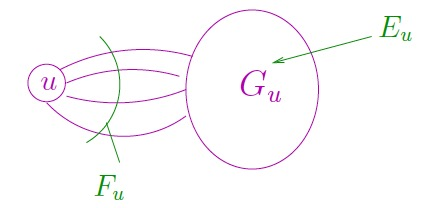
\includegraphics[width=0.4\textwidth]{vertexcover1.jpg}
\caption{Vertex Cover Substructure Lemma}\label{vertexcoverfigure}
\end{figure}
Since $S$ contains at least one endpoint for any edge in $E_u$, $S\cup\{u\}$ is a vertex cover of $G$ of size $k$.

($\Rightarrow$)
Let $S$ be a vertex cover of $G$ of size $k$. For any edge $(u,v)$, at least one of $u,v$ is inside $S$. Suppose $u\in S$. For any edge in $E_u$, at least one of its endpoints is in $S$, and it cannot be $u$, thus $S-\{u\}$ is a vertex cover of $G_u$ of size $k-1$.
\end{proof}
According to the substructure lemma, we can compute the vertex cover of a graph with Algorithm \ref{vertexcover}.
\begin{algorithm}[ht]
\caption{Vertex Cover Problem}\label{vertexcover}
\begin{algorithmic}[1]
\Input{Undirected graph $G=(V,E)$.}
\Output{Vertex cover of $G$ of size $k$.}
\If{$k=0$}
\If{$V=\emptyset$}
\State{Return $\emptyset$}
\Else\State{Fail}
\EndIf\EndIf
\State{Pick an arbitrary edge $(u,v)\in E$.}
\State{Recursively search for a vertex cover $S$ of size $k-1$ in $G_u$.}
\State{If found, return $S\cup\{u\}$.}
\State{Recursively search for a vertex cover $S$ of size $k-1$ in $G_v$.}
\State{If found, return $S\cup\{v\}$.}
\State{Fail.}\Comment{$G$ has no vertex cover of size $k$.}
\end{algorithmic}
\end{algorithm}

There are at most $O(2^k)$ recursive calls, each call takes $O(m)$ time (construction of $G_u$ or $G_v$), thus the overall running time is $O(m2^k)$, which is much better than $O(mn^k)$.

\section{Traveling Salesman Problem}
A brute-force search algorithm takes $O(n!)$ time. We will try to devise an algorithm with better running time. 

For every destination $j\in\{1,2,\dots,n\}$ and every subset $S\subseteq\{1,2,\dots,n\}$ that contains 1 and $j$, let $L_{S,j}$ represent the minimum length of a path from 1 to $j$ that visits each vertex in $S$ exactly once.
\begin{lemma}\textbf{Optimal Substructure Lemma}
Let $P$ be a shortest path from 1 to $j$ that visits each vertex in $S$ exactly once. If the last hop of $P$ is $(k,j)$ and the rest of $P$ is $P'$, then $P'$ is a shortest path from 1 to $k$ that visits each vertex in $S-\{j\}$ exactly once. 
\end{lemma}
The proof of the optimal substructure lemma is straightforward. According to the lemma, we have the induction relation
$$L_{S,j}=\min_{k\in S,k\neq j}\{L_{S-\{j\},k}+c_{kj}\}.$$
Algorithm \ref{tsp} is the dynamic programming algorithm based on this relation.
\begin{algorithm}[ht]
\caption{TSP Problem}\label{tsp}
\begin{algorithmic}[1]
\Input{A completed undirected graph with non-negative edge costs.}
\Output{$2^n\times n$ 2D array $A$ with $A[S][j]=L_{S,j}$.}
\State{Initialize $A[S][1]=\begin{cases}
0&if\:S=\{1\}\\
+\infty&otherwise
\end{cases}$}
\For{$m=2,3,\dots,n$}\Comment{$m$ = subproblem size}
\For{each $S\subseteq\{1,2,\dots,n\}$ with $\lvert S\rvert=m$ and $1\in S$}
\For{each $j\in S$ and $j\neq 1$}
\State{$A[S][j]=\min_{k\in S,k\neq j}\{A[S-\{j\}][k]+c_{kj}\}$}
\EndFor\EndFor\EndFor
\State{Return $\min_{j=2,\dots,n}{A[\{1,2,\dots,n\}][j]+c_{j1}}$}
\end{algorithmic}
\end{algorithm}
There are $n2^n$ subproblems, each of which takes $O(n)$ time. Thus the overall running time is $O(n^22^n)$.
\ifx\PREAMBLE\undefined
\end{document}
\fi